\chapter{Výsledky a porovnanie}

V tejto kapitole sa pozrieme na výkonnosť nášho riešenia v porovnaní
s CR-indexom. Testovanie prebehlo na počítači s procesorom
Intel Xeon CPU E5-2670 taktovaným na $2.60 GHz$.

Pre účely testovania sme používali dve sady vstupných dát. Prvou sadou sú
čítania získané nástrojom MiSeq z baktérie E.coli, kmeňa MG1655
získané od spoločnosti Illumina. Dĺžka genómu tejto baktérie je 4.7 miliónov bázových párov, čítania
majú viac ako $180\times$ pokrytie a chybovosť $0.75\%$. Druhú sadu tvoria čítania zo štrnásteho ľudského
chromozómu, získané z projektu GAGE \cite{gage}. Celková dĺžka reťazca je 107 miliónov bázových párov,
čítania majú $42\times$ pokrytie a chybovosť $1.5\%$.

Okrem týchto dvoch sád čítaní sme použili aj simulované čítania náhodne generované z osekvenovaného
genómu baktérie E.coli s rôznou dĺžkou aj chybovosťou.

Testovali sme rýchlosť hľadania čítaní s daným podreťazcom a veľkosť štruktúr, ktoré potrebujeme pre odpovedanie
na takéto dotazy za rôznych podmienok. Pokiaľ nie je povedané inak, hodnota $k$ je $20$.

Podreťazce pre dotazy sme generovali tak, aby $95\%$ podreťazcov
pochádzalo z náhodných čítaní a zvyšných $5\%$ boli úplne náhodné reťazce.

\begin{figure}

\centerline{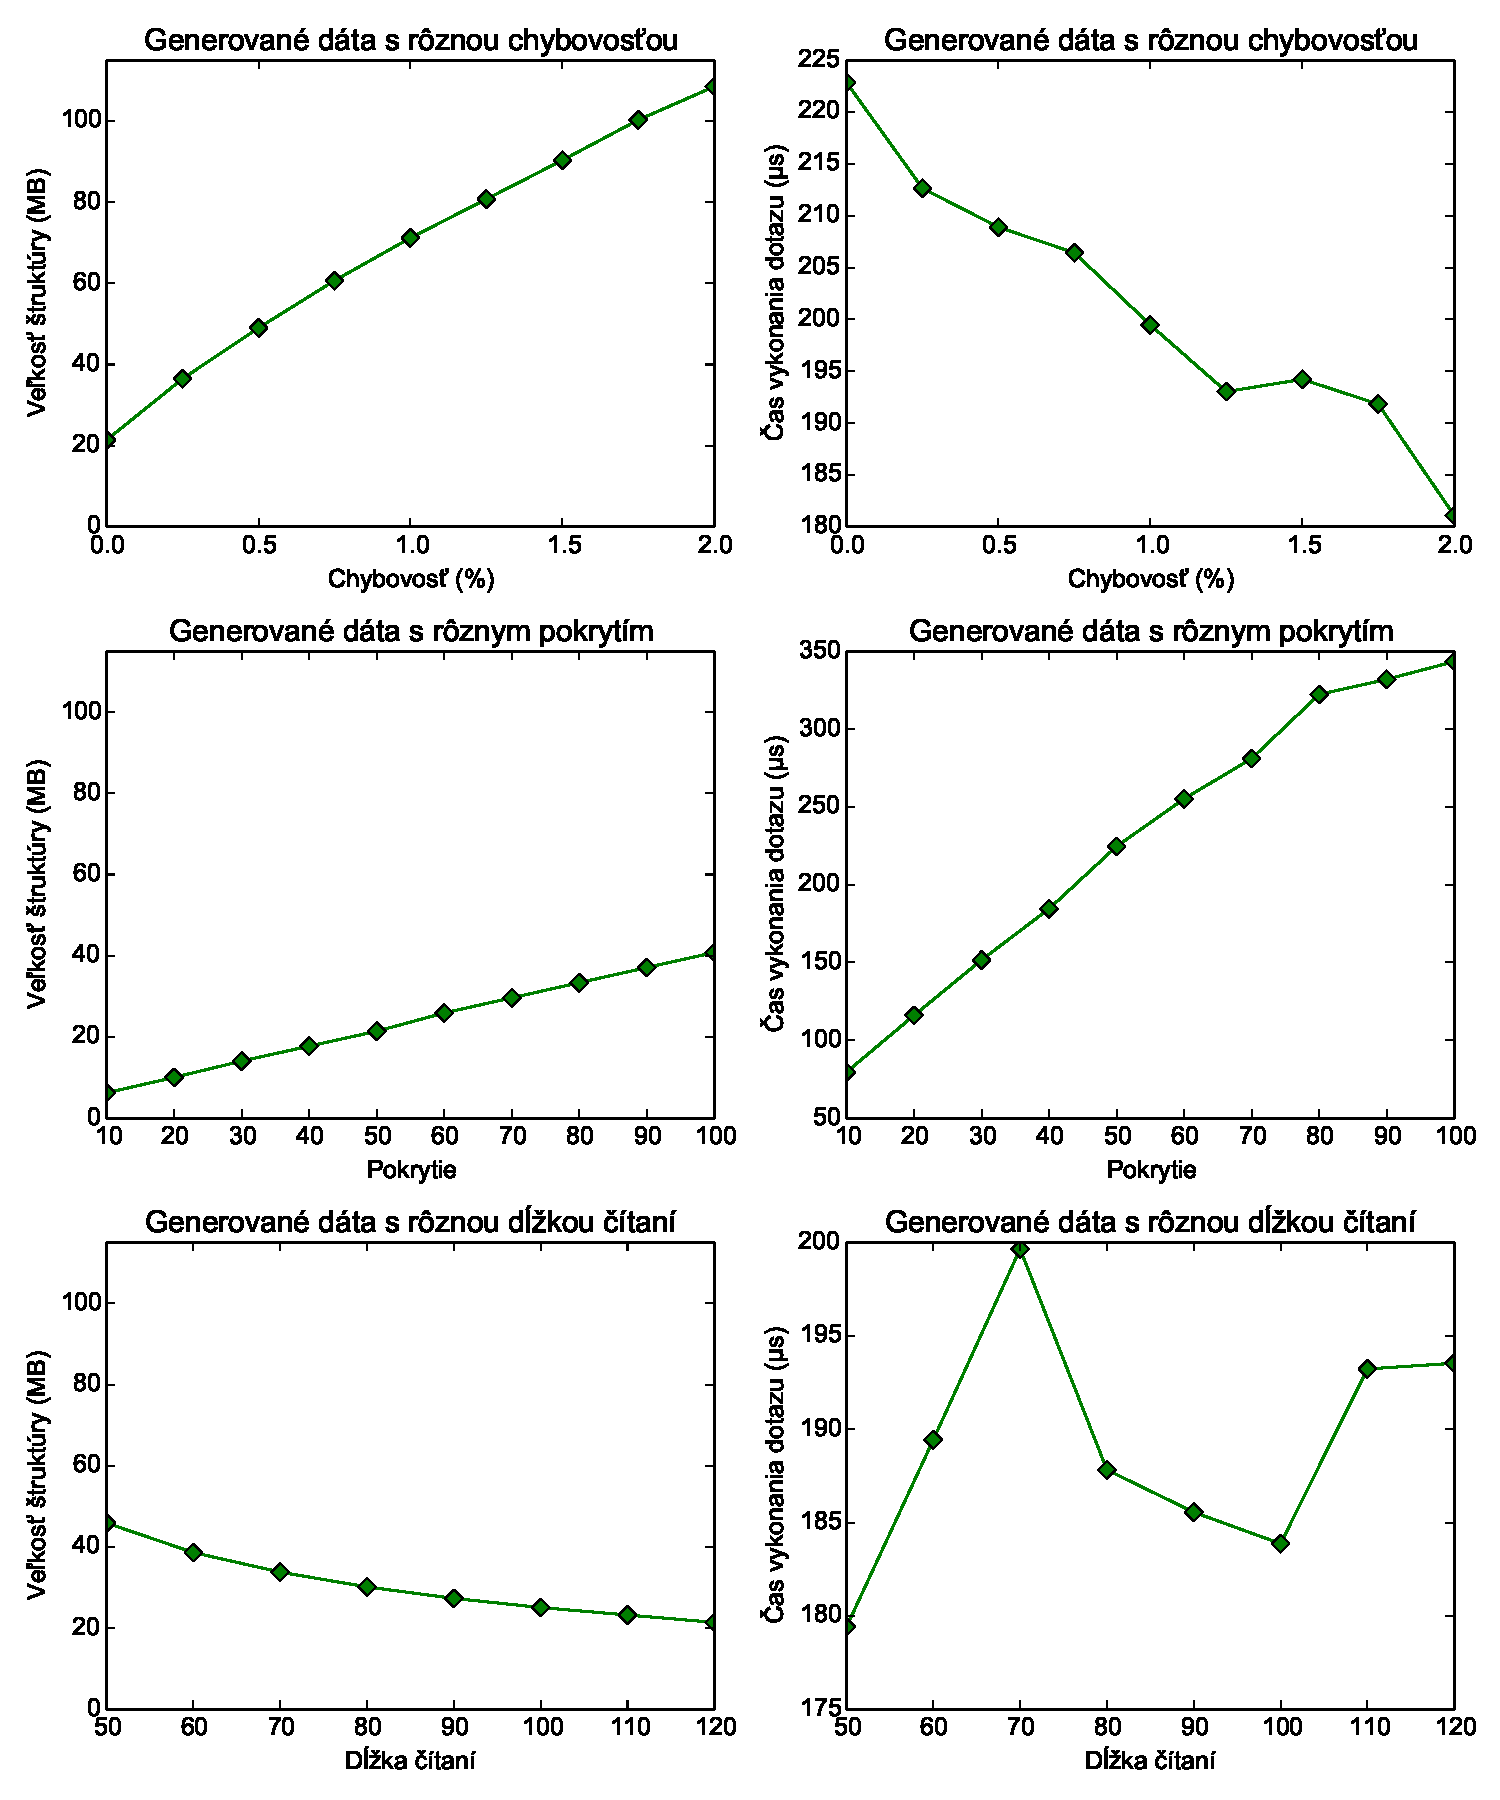
\includegraphics[width=1\textwidth]{images/chart_artificial.pdf}}

\caption[Simulované dáta]{Panely A a B: vplyv chybovosti dát na rýchlosť vykonávania dotazu a množstvo
pamäte potrebnej na uloženie všetkých pomocných štruktúr. Panely C a D: vplyv pokrytia.
Panely E a F: vplyv dĺžky čítaní. Pri druhej a tretej dvojici panelov boli dáta generované
bez chýb.}

\label{chart:artificial}

\end{figure}

\section{Generované dáta}

Obrázok \ref{chart:artificial} prezentuje výsledky pre simulované dáta. Ako prvé sme
generovali čítania dĺžky $120$ s rôznou šancou na chybné určenie bázy (panely A a B). Čítania mali
$50\times$ pokrytie. Ako druhé sme generovali čítania s rôznym pokrytím bez chýb (panely C a D).
Na záver sme generovali čítania s $50\times$ pokrytím, líšiace sa v dĺžke
čítaní (panely E a F).

Prvý experiment (panely A a B) ukazuje, že vyššia chybovosť spôsobuje zásadné zväčšenie celej štruktúry, ale
čas na vykonanie dotazu klesá. Za nárast pamäťovej náročnosti môžu dve skutočnosti. Prvou
je predĺženie $k$-nadslova, ktoré musí obsahovať všetky $k$-tice s chybou. Druhou je zväčšený
počet začiatkov, ktorý je spôsobený tým, že $k$-tice s chybou v čítaní sú oddelené od zvyšku
bez chyby. Za mierne zrýchlenie dotazov pri väčšej chybovosti je pravdepodobne zodpovedné
predĺženie $k$-nadslova, kvôli ktorému sa zníži priemerný počet začiatkov na pozíciu
v $k$-nadslove.

Na paneloch C a D vidíme, že vyššie pokrytie navyšuje aj pamäťové, aj časové nároky.
Pri každom pokrytí bola dĺžka $k$-nadslova takmer rovnaká, navyšoval sa iba počet začiatkov.
Z tohto dôvodu stúpal priemerný počet začiatkov na znak v $k$-nadslove, čím si vysvetľujeme
vyšší čas potrebný na vyriešenie dotazu.

V poslednej dvojici panelov E a F vidíme, že dlhšie čítania sa našim postupom uložia na menej
miesta. Toto je spôsobené tým, že sa zmenší počet začiatkov. Zmeny v čase potrebnom na
riešenie dotazu sú malé a vysvetľujeme si ich ako náhodný šum.

\begin{figure}

\centerline{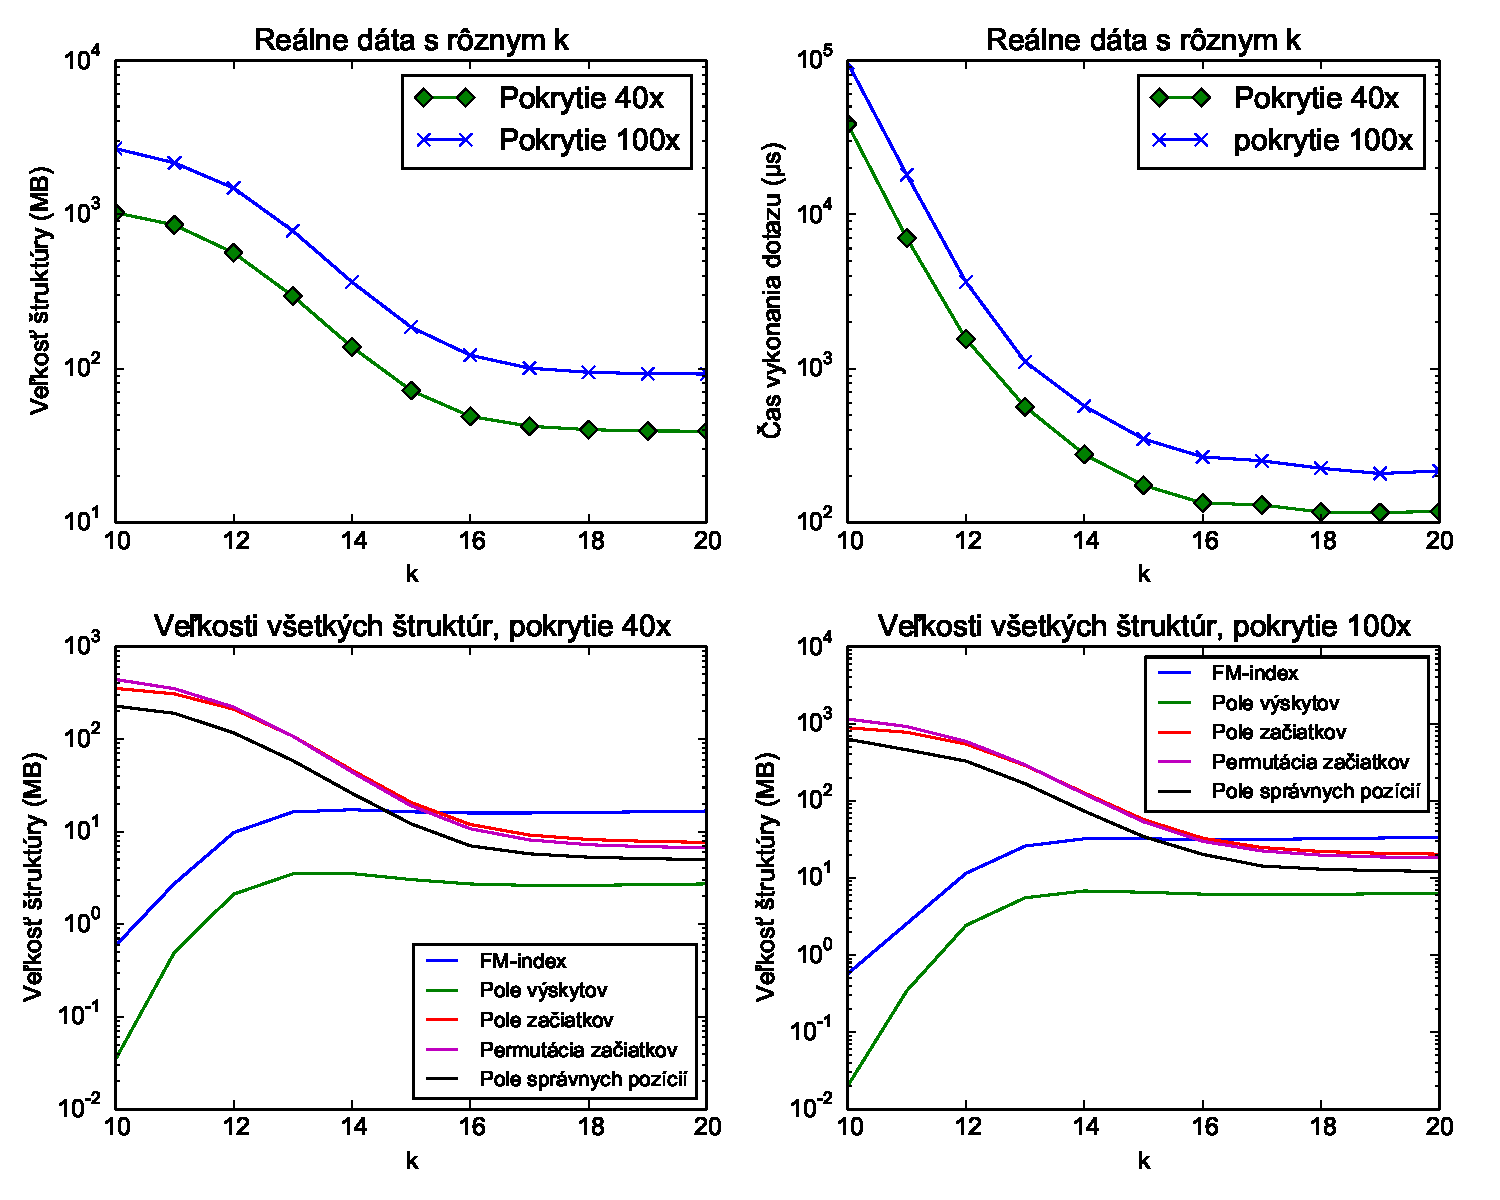
\includegraphics[width=1\textwidth]{images/chart_difks.pdf}}

\caption[E.coli dáta s rôznym $k$]{Výsledky testovania na čítaniach baktérie E.coli pre rôzne $k$.
Panely A a B: vplyv hodnoty $k$ na
pamäťové nároky štruktúry a čas spracovávania dotazu. Panel C: veľkosti
jednotlivých polí a štruktúr, ktoré používame, v závislosti od $k$ pri $40\times$ pokrytí.
Panel D: veľkosti štruktúr pri $100\times$ pokrytí. Kvôli veľkému rozsahu nameraných hodnôt sú veľkosti
aj čas udávané v logaritmickej škále.}

\label{chart:difks}

\end{figure}

\section{Rôzne $k$}

Na druhej sade testov si ukážeme, aký vplyv má hodnota $k$ na veľkosť a rýchlosť celej štruktúry (obr. \ref{chart:difks}).
Tentokrát sme použili podmnožinu čítaní pre baktériu \emph{E.coli} so $40\times$ a $100\times$ pokrytím.

Pre malé hodnoty $k$ máme vysokú pravdepodobnosť, že sa rôzne časti genómu budú zhodovať v $k$-ticiach.
Zatiaľ čo dĺžka $k$-nadslova je rekordne malá, jednotlivé
čítania sú roztrúsené po tomto $k$-nadslove, čo má za efekt veľmi veľký počet začiatkov.

Pre rastúce
$k$ spočiatku rastie dĺžka nadslova, až sa pri $k \ge 15$ ustáli na takmer rovnakej hodnote. Zároveň
môžeme pozorovať, že pre $k \ge 16$ sa takmer vôbec nemení ani počet začiatkov. Tento fakt si
vysvetľujeme tak, že pre takéto $k$ začína $k$-nadslovo pomerne dobre reprezentovať celý genóm
\emph{E.coli}. Rovnako ako s rastúcim $k$ klesá počet začiatkov, klesá aj čas spracovávania dotazu, čo len
potvrdzuje, že táto rýchlosť závisí od počtu skontrolovaných potenciálnych začiatkov.

\begin{figure}

\centerline{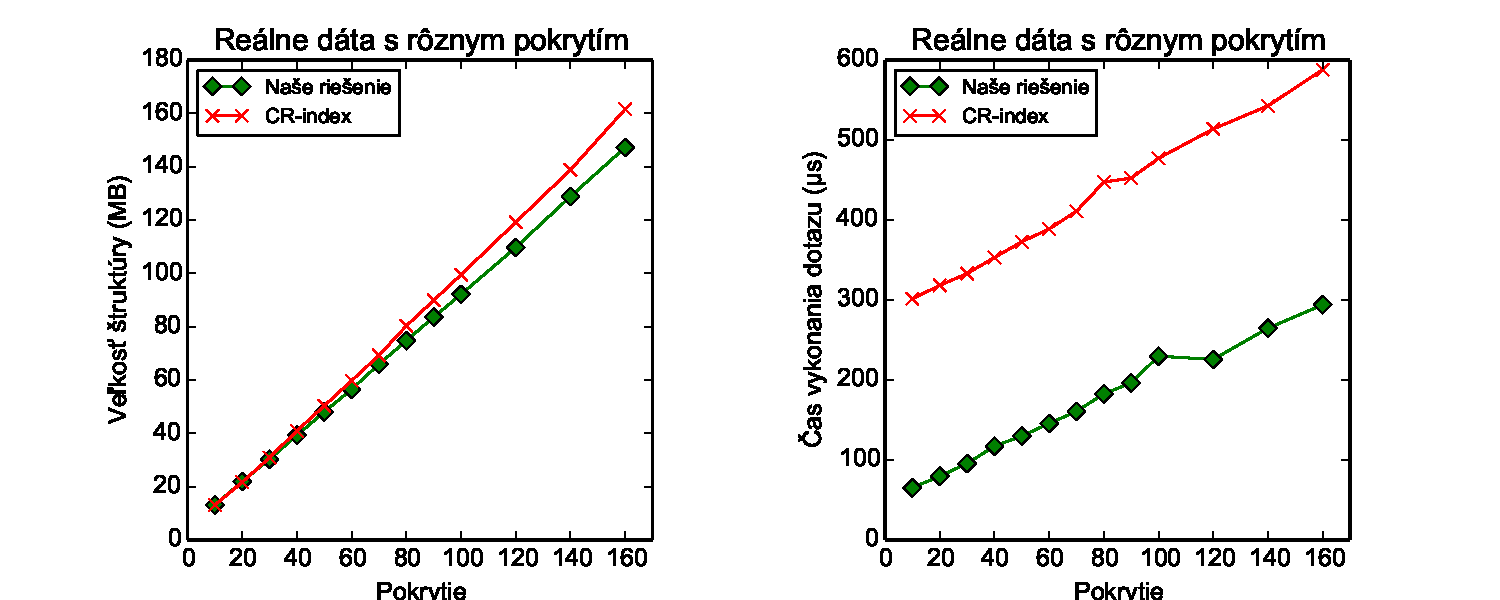
\includegraphics[width=1\textwidth]{images/chart_srcr.pdf}}

\caption[Porovnanie CR-indexu a našej štruktúry]{Porovnanie pamäťovej a časovej náročnosti
CR-indexu a nášho riešenia na čítaniach baktérie E.coli pri rôznom pokrytí.}

\label{chart:srcr}

\end{figure}

\begin{figure}

\centerline{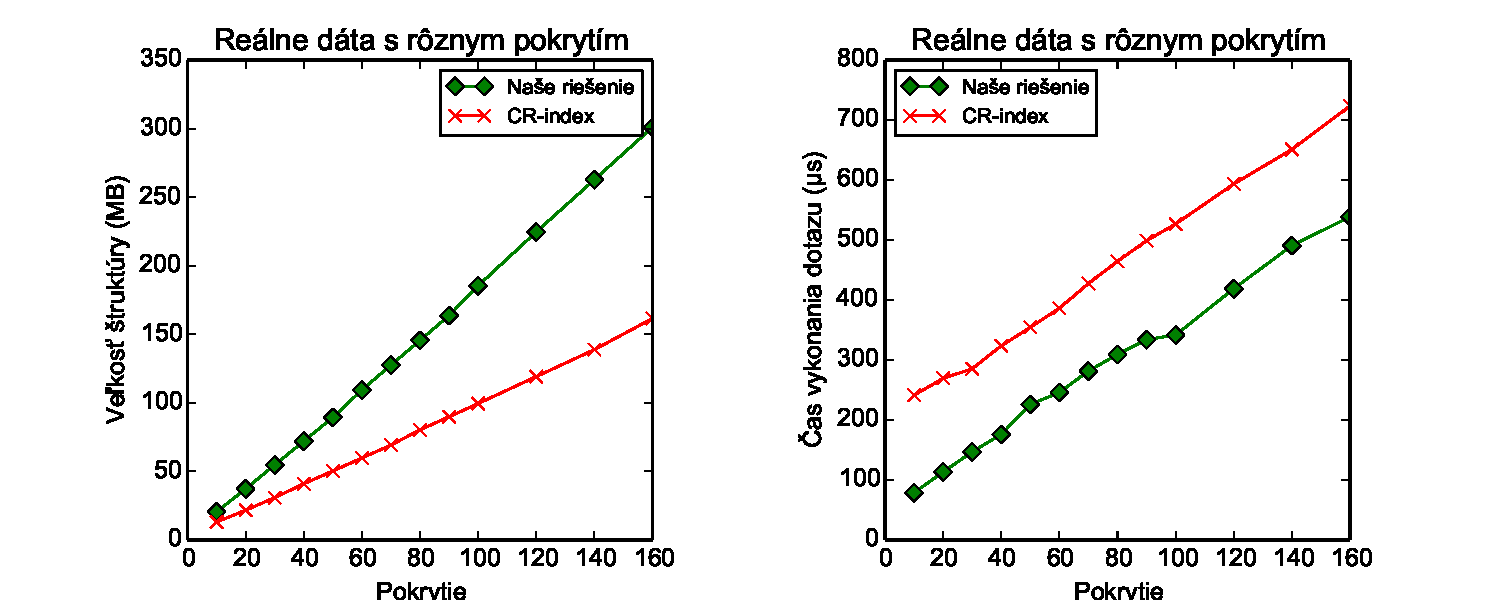
\includegraphics[width=1\textwidth]{images/chart_srcr_15.pdf}}

\caption[Porovnanie CR-indexu a našej štruktúry pre $k = 15$]{Porovnanie pamäťovej a časovej náročnosti
CR-indexu a nášho riešenia na čítaniach baktérie E.coli pre $k=15$ pri rôznom pokrytí.}

\label{chart:srcr_15}

\end{figure}


\section{Porovnanie s CR-indexom}

Ako posledné si ukážeme porovnanie nášho riešenia s CR-indexom na obr. \ref{chart:srcr}.
Z čítaní z baktérie \emph{E.coli} sme náhodne povyberali podmnožiny s daným pokrytím. Pri každom
pokrytí používalo naše riešenie o trochu menej pamäte, napriek tomu bolo o viac než $200\mu s$
rýchlejšie. Na obr. \ref{chart:srcr_15} zas môžeme pozorovať, že pre menšie hodnoty $k$ je
síce naše riešenie rýchlejšie, ale vyžaduje zhruba dvakrát viac pamäte, než CR-index.
Pre menšie $k$ môžeme predpokladať, že CR-index bude ešte o trochu rýchlejší, naše riešenie
bude ešte pomalšie kvôli väčšiemu množstvu začiatkov.

Podobne sme otestovali oba programy na čítaniach z ľudského chromozómu 14. CR-index na týchto čítaniach
potreboval $1.2GB$ pamäte, naša štruktúra potrebovala až vyše $2.1GB$. Z časového hľadiska
to vyšlo naopak, CR-index potreboval okolo $21ms$ na spracovanie dotazu, naša štruktúra
to zvládla v priemere za $9ms$.

\section{Zhrnutie}

So zvyšujúcou sa hodnotou $k$
veľkosť štruktúry klesá a jej rýchlosť stúpa. Očakávame však, že pre dostatočne veľké $k$ začne byť
dĺžka nadslova dominantným faktorom vo veľkosti celej štruktúry a teda celková pamäťová
zložitosť začne stúpať. Jedným
z možných smerov ďalšieho vývoja je podpora pre dotazy kratšie než $k$, vďaka ktorej sa možno
budú dať využiť pamäťové a časové výhody väčšieho $k$ aj pre kratšie dotazy.

Ďalšie pozorovanie je, že so zvyšujúcou sa chybovosťou narastá veľkosť štruktúry.
S týmto by sme sa mohli vysporiadať podobne, ako CR-index. Očakávame však, že použitím
riešenia z CR-indexu stratíme náskok v rýchlosti.

Ďalšie pozorovanie je, že zatiaľ čo s malým $k$ je dĺžka $k$-nadslova pomerne malá, na
reprezentáciu čítaní potrebujeme veľmi veľa pamäte. Pre väčšie $k$ sa pomery obrátia,
$k$-nadslovo bude väčšie, zatiaľ čo začiatky budeme vedieť reprezentovať v oveľa menšej pamäti.
Z tohto vyplýva, že naše riešenie je efektívne hlavne v špeciálnych prípadoch, keď
je krátke $k$-nadslovo a počet začiatkov je malý.

Pri porovnaní s CR-indexom bolo naše riešenie pre stredne veľké $k$ rýchlejšie, túto
skutočnosť pripisujeme spôsobu, akým sa CR-index vysporadúva s chybami. Zatiaľ čo
CR-index pre každý dotaz na podreťazec $r$ hľadá veľké množstvo reťazcov, ktoré je možné
získať úpravou jedného znaku, naše riešenie hľadá iba jeden.

Pre malé $k$ je naše riešenie pomerne neefektívne, pokiaľ nás zaujímajú čítania obsahujúce
dotazovaný podreťazec. Napriek tomu môže byť použiteľné aj pre takéto $k$, pokiaľ bude
podporovať iba dotazy na počty výskytov.
